% Version 2019-01-08
% update – 161114 by Ken Arroyo Ohori: made spacing closer to Word template throughout, put proper quotes everywhere, removed spacing that could cause labels to be wrong, added non-breaking and inter-sentence spacing where applicable, removed explicit newlines
% update – 010819 by Dennis Wittich: made spacing and font size closer to Word template, updated references and refernces style
% update – 042319 by Dennis Wittich: font size of captions set to 'small', first author names are shortened, hyphenation fixed

\documentclass{isprs} % isprs class modified 23-04-2019 (Dennis Wittich)
\usepackage{subfigure}
\usepackage{setspace}
\usepackage{geometry} % added 27-02-2014 Markus Englich
\usepackage{epstopdf}
\usepackage[labelsep=period]{caption}  % added 14-04-2016 Markus Englich - Recommendation by Sebastian Brocks
\usepackage[british]{babel} 

\geometry{a4paper, top=25mm, left=20mm, right=20mm, bottom=25mm, headsep=10mm, footskip=12mm} % added 27-02-2014 Markus Englich
%\usepackage{enumitem}

%\usepackage{isprs}
%\usepackage[perpage,para,symbol*]{footmisc}

%\renewcommand*{\thefootnote}{\fnsymbol{footnote}}
\captionsetup{justification=centering,font=normal} % thanks to Niclas Borlin 05-05-2016
\captionsetup[figure]{font=small} % added 23-04-2019 Dennis Wittich
\captionsetup[table]{font=small} % added 23-04-2019 Dennis Wittich

\begin{document}

\title{SMODERP2D SOIL EROSION MODEL ENTERING AN OPEN SOURCE ERA WITH
  GPU-BASED PARALLELIZATION}

% KAO: Remove extra spacing
\author{
 M. Landa\textsuperscript{1}, J. Jeřábek\textsuperscript{2}, O. Pešek\textsuperscript{1}, P. Kavka\textsuperscript{2}}

% KAO: Remove extra newline
\address{
  \textsuperscript{1 }Dept.\ of Geomatics, Faculty of Civil Engineering, Czech Technical University in Prague,\\ Czech Republic - (martin.landa, ondrej.pesek)@fsv.cvut.cz\\
  \textsuperscript{2 }Dept.\ of Landscape Water Conservation, Faculty of Civil Engineering, Czech Technical University in Prague,\\ Czech Republic - (jakub.jerabek, petr.kavka)@fsv.cvut.cz\\
}

% If the corresponding author is NOT the final author, always add a % space before the subsequent comma, i.e.
% first author name\textsuperscript{a,}\thanks{Corresponding author} , % second author name \textsuperscript{b}, etc.
% thanks to Niclas Borlin 05-05-2016


\commission{VI, }{VI} %This field is optional.
\workinggroup{VI/4} %This field is optional.
\icwg{}   %This field is optional.

% KAO: Use times symbol
\abstract{ SMODERP2D is a runoff-soil erosion physically-based
  distributed episodic model used for calculation and prediction
  processes at agricultural areas and small watersheds. The core of
  the model is a raster based cell-by-cell mass balance calculation
  which includes the key hydrological processes, such as effective
  precipitation, surface runoff and stream network routing. Effective
  precipitation, the forcing of the runoff and erosion processes, is
  reduced by surface retention and infiltration. Surface runoff
  consists of two components: slower sheet and concentrated rapid rill
  flow. Stream network routing is performed line-by-line in user
  predefined polyline layer.

  SMODERP is a long-term running project driven by the Department of
  Landscape Water Conservation at the Czech Technical University in
  Prague. At the beginning SMODERP has been developed as a surface
  runoff simulated by profile model (1D). Later the model has been
  redesigned using spatially distributed method. This version is named
  SMODERP2D. Ongoing development is focused on obtaining parameters of
  the hydrological models, incorporating new infiltration and flow
  routing routines, and conceptualization of a rill flow and rill
  development. The model belongs to a family of so called GIS-based
  hydrological models utilizing capabilities of GIS software for
  geodata processing. Importantly, the SMODERP2D project is currently
  entering the open source world. Originally the model could be run
  only in proprietary Esri ArcGIS platform. A new version of the model
  presented by this manuscript adds support for two key open source
  GIS platforms, GRASS GIS and QGIS. A newly developed GRASS module
  and QGIS plugin significantly increases accessibility of the
  SMODERP2D model for research purposes and also for engineering
  practice.

  Middle scale distributed hydrological models often encounter with a
  high computation costs and long model runtime. Long runtime is
  caused by high resolution input data which is easily available
  nowadays. The project also includes an experimental version of the
  SMODERP2D model enabling the parallelization of computations. This
  parallelization is done using TensorFlow, and its goal is to
  decrease the time needed for its run. It is supported by both CPU
  and GPU. Parallelization of computations is an important step
  towards providing SMODERP2D web processing services in order to
  allow quick and easy integration to highly specialized platforms
  such as Atlas Ltd.  }

\keywords{Hydrology, Soil Erosion Models, GIS, Open Source, Parallel computing}

\maketitle

%\saythanks % added 28-02-2014 Markus Englich

\section{INTRODUCTION}\label{INTRODUCTION}
 
% KAO: Sloppy spacing ensures non-overfull lines. Can be removed if this is not an issue.
\sloppy

Erosion / hydrological models (EH) are being used for various research or engineering purposes. 
Results of such models may be used as input information for planning 
or designing soil conservation measures in the landscape and hydrological units - basins. 
Runoff water volume and transported soil amounts
or discharge time series are being calculated
in order to design the protection measures sufficient for a given flood 
or soil transport event. Another example of a practical 
application of EH models may be land-use change or build up areas development studies 
or effect of those on water or soil transport regime. 
Great use of EH models is also in extreme event 
forecasting. In research, EH models 
are being used to proof a new theory or to test hypotheses related 
to mechanism controlling the runoff and soil transport.

Empirical erosion models are often based on Universal Soil Loss Equation (USLE), 
\cite{wischmeier1978,renard1997} and empirical hydrological models on the Curve 
number method (CN) \cite{cronshey1986}, concepts more than 30 years old. 
Using empirical approaches may introduce limitations in the protection measures design e.g. 
because mentioned models do not take into account the transient nature of modelled processes. 
Physically based models are being developed to overcome the empirical models limitations. 

Processes taking place in a landscape are spatially distributed, which is the reason why GIS 
is often deploying in the modelling process taking advantage 
of ready to use GIS features. EH models have similar structure 
(although each model is specific in terms in processes solved, 
its purpose or coding strategy). The forcing of the runoff and soil loss is precipitation
which is often introduced in the model in spatially distributed 
manner. Majority of models include an infiltration routine with 
spatially distributed parameters, since grassland 
and parking lot may be presented in a single hydrological model 
and have vastly distinct infiltration characteristic. Infiltrated 
water is transported to the soil which has varying transport properties. 
Ponging water creates overland flow which leads to soil transport 
and may cause severe soil and nutrition losses in the landscape. 
Linear (water courses, streets, ditches) 
or points (typically a water pump) features may be presented  
in the modelled system and affect the water flow or soil transport regime. 
GIS software has tools to operate with the linear and point features, 
and spatial data which simplifies modellers live.

The EH model may encounter with some run-time issues which 
rise from model spatial and temporal discretization. 
Data availability and larger computation resources lead more often 
to the use of finer spatial resolution. 
It was noted in \cite{molnar2000} that raster grid cell size is interchangeable 
in terms of spatial discretization if the model parameters 
were calibrated on the model with the same raster grid size. 
Finer spatial resolution, in some 
cases, causes problems with time discretization and the time step size. 
Time step size is commonly 
controlled with Courant–Friedrichs–Lewy (CFL) criterion~\cite{courant1928}. 
CFL criterion force the time step to decrease if: a) velocity of flow 
process increases or; b) the spatial discretization becomes finer. 
Maximum acceptable CFL value, which preserves computation stability, theoretically equals one. 
For shallow surface processes (processes which take place in the used model)
CFL criterion should 
be even smaller than one as it was noted in \cite{zhang1989}
or \cite{esteves2000}. The need for smaller than one CFL criterion 
is caused mainly by the discrepancy between solution (surface water height), 
cell size and surface roughness coefficient 
or by sharp surface slope changes between adjacent cells. 

In case of EH models, the commonly computed processes are sheet 
and 
rill flow. 
The sheet flow covers the earth's surface evenly, whereas rill flow detaches 
the soil material and concentrates its flow in the created rill 
(therefore it is also called concentrated flow).
Although the concentrated rill flow is particularly fast (causing  
the time step size constraint) it usually occupies a small portion of the area. 
The computation may end up in a situation where a 
small portion of the computed area demands a shorter time step 
(due to rill flow presence ) whereas the rest of the area allows larger time step. 
In that case, only a small part of the computed area with developed rills causes the long model run-time. 

To summarize and outline the objectives of this manuscript. The advantage of high-resolution
geodata availability is constrained with the increasing computation demands
of the calculation. In the case of this manuscript, the extremely 
short time steps caused by the needs of CFL criterion is the main concern. 
Not all computed processes need shorter time step and processes which do are spatially limited (the concentrated flow in rill). 
In other words, 
the whole basin computation run-time is being increased due to small part
of the computed basin. One way to overcome this problem is to use 
GPU or CPU palatalization. In this manuscript, TensorFlow Python library 
\cite{tensorflow2015-whitepaper} was tested to parallelize the EH model. 
Besides the TensorFlow a CPU parallelization is outlined. 
The testing was performed with the SMODERP2D EH model. The model calculates the surface runoff
and soil loss processes with the use of GIS software for the data pre- and postprocessing. 
GRASS GIS provider and QGIS plugin were lately implemented in the SMODERP2D project, next to the already existing ESRI ArcGIS plugin. 
Those new features and some of the used principles used in the SMODERP2D model are also presented in this paper. 

% Nevýhoda -  Výpočet je numericky náročný, kuli CFL
% Procesy jsou rychlé jen v některých buňkách, ostatní části “čekají”
% Jedním z přístupů je využití rozbusnosti výpočetní techniky. 
% TO je umožněno paralezlazcí výpočtu (CPU/GPU). Princip pravidelné mřížky -  nejsnazší, princip      subpovodí     
% Testování jak využít paralelizaci je testováno na modelu SMODERP..


\section{MATERIAL AND METHODS}\label{sec:mat_met}

\subsection{SMODERP2D model}
The SMODERP2D model has been integrated in open source 
GIS packages and tested for the GPU/CPU parallelization
with in presented work. The model, which is now capable of 2D
calculation, has been developed from the 1D profile version~\cite{Holy1984}. 
Description of the model follows.

The model has a simple structure based on the mass balance equation:
\begin{equation}\label{equ:mass_bal}
    \frac{Storage}{\Delta t} = \nonumber  
    Inflow - Outflow
\end{equation}
where {\it Storage} represents 
surface water level $h$ [$L$] which changes each proceeding time
during the computation. $Inflow$ and $Outflow$ terms on the right-hand side of
the equation~(\ref{equ:mass_bal}) represent the water flowing in and out the storage 
during the time step ${\Delta t}$ and consist of several components.
The $Inflow$ and $Outflow$ of $i_{th}$ raster cell are defined as:
\begin{equation}\label{equ:inflow}
    Inflow_i = es_{i} + \sum_j^n q_{j}
\end{equation}
\begin{equation}\label{equ:outflow}
    Outflow_i = inf_{i} - q_{i} - ret_i
\end{equation}
\begin{tabbing} 
where \hspace{0.6cm} \= $es$ = effective precipitation\\
\> $q$ = inflow to resp. outflow from a given raster cell\\
\> $inf$ = infiltration\\
\> $ret$ = surface retention for a given raster cell
\end{tabbing}
The sum $\sum_j^n$ in expression~(\ref{equ:inflow}) represents sum of all inflows to the cell $i$. 
The flow direction and therefore the sum $\sum_j^n$
is controlled by D8 flow direction algorithm~\cite{ocallaghan1984}.  Effective
precipitation $es$ is potential precipitation reduced by
interception of the rainfall water on the vegetation.

The model is forced to satisfy the Courant--Friedrichs--Lewy (CFL)
criterion~\cite{courant1928}:
\begin{equation}\label{equ:CFL}
    CFL = \frac{q\textrm{d}t}{\textrm{d}x} < 1.0
\end{equation}
\begin{tabbing} 
where \hspace{0.6cm} \= $\textrm{d}t$ = time step\\
\> $\textrm{d}x$ = grid cell size
\end{tabbing}
If the flow $q$ is high, the model is forced to decrease the
time step in order to satisfy the CFL criterion, since a grid cell size
is fixed.

The flow $q$ in the equations~(\ref{equ:inflow}) and~(\ref{equ:outflow})
has two components. Slower and spatially extensive sheet flow
$q_{sh}$:
\begin{equation}\label{equ:sheetflow}
    q_{sh} = XI^Yh^b
\end{equation}
\begin{tabbing} 
where \hspace{0.6cm} \= $X,Y,b$ = empirical parameters\\
\> $I$ = surface slope
\end{tabbing}
and faster concentrated rill flow $q_{rl}$ calculated by the Mannings formula:
\begin{equation}\label{equ:rillflow}
    q_{rl} = A\frac{1}{n} R^{2/3} I^{1/2}
\end{equation}
\begin{tabbing} 
where \hspace{0.6cm} \= $A$ = cross-section area\\
\> $n$ = roughness in the rill\\
\> $R$ = hydraulic radii
\end{tabbing}
The resulting flow is a sum of sheet and rill flow:
\begin{equation}\label{equ:flow}
    q = q_{rl} + q_{rl}
\end{equation}
The sheet flow starts when the infiltration capacity is exceeded; 
when rainfall is higher than infiltration. The rill flow emerges if 
a critical water level of sheet flow is exceeded. The critical 
water level is defined based on critical shear stress; when the 
drag force of the flowing water becomes large than the cohesive 
forces of the soil particles.
From the definition, the sheet flow does not occur all over the 
basin area. The rill flow is usually presented to even lower extend. 
However, the CFL criterion is more likely constrained by the 
rapid rill flow even though its it occupy smaller area compared to sheet flow. 

Infiltration is solved with Phillip's infiltration equation \cite{philip1957theory}:
\begin{equation}\label{eq:Phillips}
    inf = 1/2St^{-1/2} + Ks
\end{equation}
\begin{tabbing} 
where \hspace{0.6cm} \= $S$ = sorptivity\\
\> $K_s$ = hydraulic conductivity
\end{tabbing}

Parameters of relations~(\ref{equ:sheetflow})~(\ref{equ:rillflow}) and
(\ref{eq:Phillips}) are in most cases spatially distributed. It is 
therefore beneficial to incorporate GIS packages in the modeling process. 





\subsection{SMODERP2D entering an open source world}\label{ref:open_source_providers}

SMODERP2D is the project with a long history. Over the years its
development has been driven by the Department of Landscape Water
Conservation at the Czech Technical University in Prague. In 2018
SMODERP2D developers started working on a new generation of the model
in order to solve or at least to improve various critical issues of
the project (see SMODERP2D logo in Figure~\ref{fig:smoderp2d_logo}). 
This includes most importantly the computation stability
and performance, better interoperability, and lack of
documentation. Recently SMODERP2D source code has been published on
GitHub \cite{smoderp2d-github-2019} under GNU GPL licence in order to
attract a wider audience, new developers and users.

\begin{figure}[ht!]
  {\tiny
\begin{verbatim}

       @ @ @   @       @     @ @     @ @ @     @ @ @ @  @ @ @    @ @ @
      @        @ @   @ @   @     @   @     @   @        @     @  @     @
      @        @   @   @  @       @  @      @  @        @     @  @     @
        @ @    @       @  @       @  @      @  @ @ @    @ @ @    @ @ @
            @  @       @  @       @  @      @  @        @   @    @
            @  @       @   @     @   @     @   @        @    @   @
       @ @ @   @       @     @ @     @ @ @     @ @ @ @  @     @  @

      \  \  /   / /    \   \  /   \  /    /     /        @ @ @   @ @ @
       \ _\/   /_/      \   \/     \/    /_____/        @     @  @     @
           \__/          \  /      _\___/                     @  @      @
               \____      \/      /                          @   @      @
                    \_____/______/                         @     @      @
                                 \                       @       @     @
                                  \____________________ @ @ @ @  @ @ @
\end{verbatim}
}
\caption{ASCII-art SMODERP2D project logo}
\label{fig:smoderp2d_logo}
\end{figure}

The model is implemented in Python programming language using the
object-oriented paradigm. The original source code has been designed
with a low level of scalability, limited readability and
interoperability. Part of the computation phase responsible for a data
preparation was restricted to a single platform only, Esri ArcGIS. In
2018 the original source code has been completely refactorized. Python
classes defining computational steps were re-organized in a
hierarchical manner. Major design-related changes have been done in
Python classes responsible for data handling and preparation using GIS
software tools. Data preparation workflow is handled by a
newly-defined a base, partly abstract Python class ({\tt BaseProvider}
in Figure~\ref{fig:uml_diagram}). Functionality depending on used
GIS package has been separated into new classes. This step was crucial
in order to make data preparation workflow GIS package
independent. The only supported platform, Esri ArcGIS, has been
separated from a base workflow. Based on that, a new concept of
so-called {\em GIS providers} has been introduced, see
Figure \ref{fig:uml_diagram}. 

\begin{figure}[ht!]
  \begin{center}
    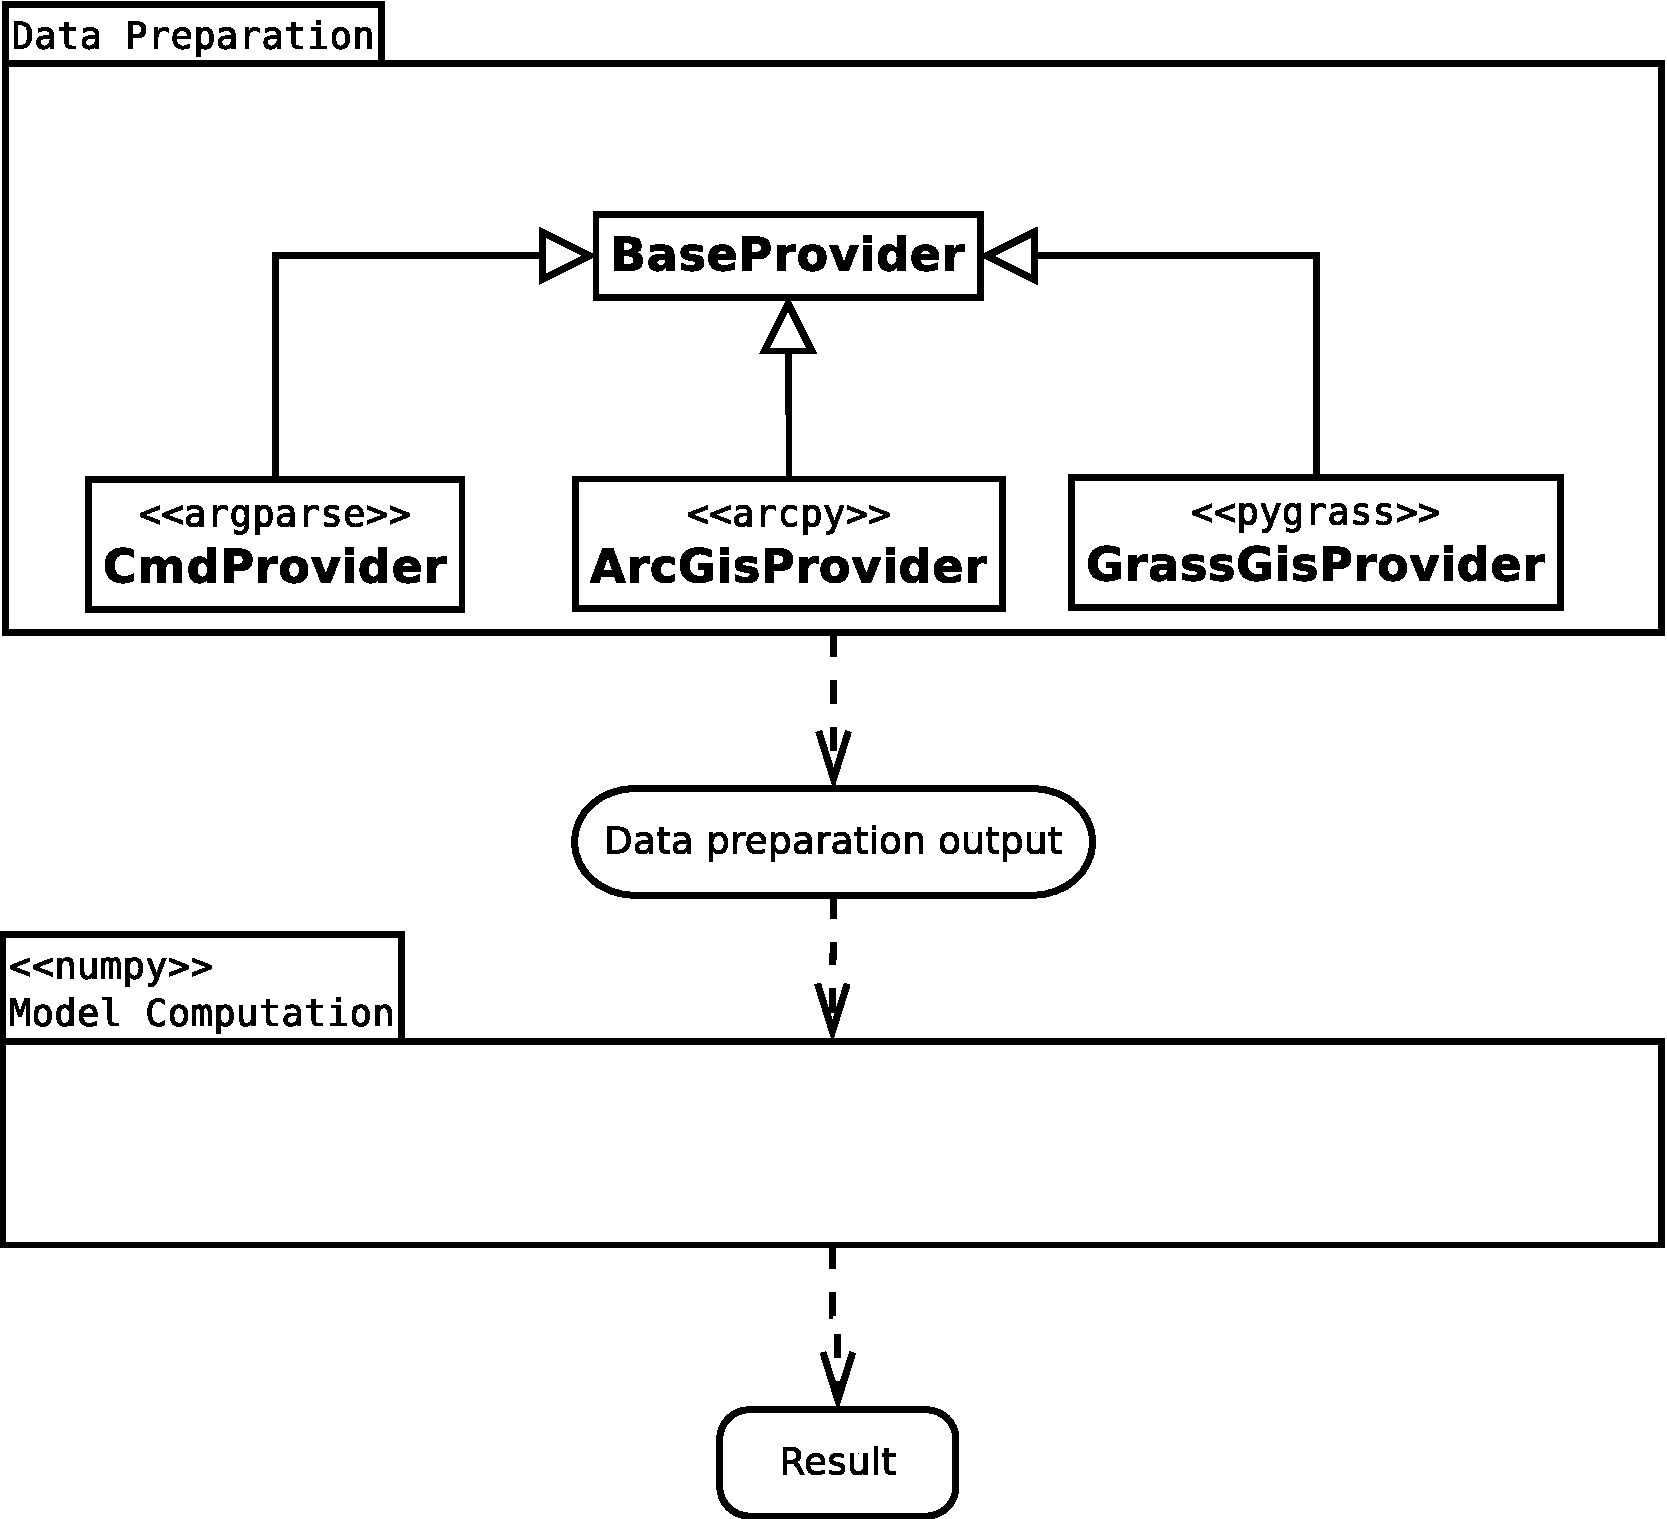
\includegraphics[width=0.8\columnwidth]{figures/uml_diagram.pdf}
    \caption{Concept of GIS providers (software dependecies outlined by stereotypes)}
    \label{fig:uml_diagram}
  \end{center}
\end{figure}

The key point is the separation of GIS functionality related code from
the~generic workflow defined by the base provider. The base provider
depends only on standard builtin Python libraries. Array-like
computation is performed by a well-known NumPy library. Using GIS
provider prototypes, the SMODERP2D project can be easily extended to
support other GIS packages. Currently, the SMODERP2D project comes
with three different GIS providers. Support for Esri ArcGIS platform
is implemented by {\tt ArcGISProvider}, GRASS GIS is handled by {\tt
  GrassGisProvider}, see \ref{sec:grass_provider}. The {\tt
  CmdProvider} is triggered only when the model computation is run
from a command-line. In this case, it is assumed that the data
preparation phase has been already performed by one of supported GIS
platforms.

Example of running computation from a command-line bellow. Option {\it
  --typecomp roff} specifies that only model computation without data
preparation phase is triggered. It means that data has been already
preprocessed and stored in a pickle file distributed by a {\it test.ini}
configuration file.

\begin{verbatim}
python ./bin/start-smoderp2d.py --typecomp roff \
 --indata tests/test.ini
\end{verbatim}

\subsubsection{GRASS GIS integration}\label{sec:grass_provider}
SMODERP2D supported GIS platforms have been recerently extended by a
+new GRASS-based GIS provider. Introducing an open source GIS platform
to SMODERP2D workflow is crucial from the perspective of
interoperability. SMODERP2D users can choose between a proprietary
Esri ArcGIS platform and an open source GRASS GIS
\cite{neteler2012grass}. The GRASS GIS provider is designed similarly
to ArcGIS provider. From a Python perspective, there is only one
difference, GIS functions are accessed by PyGRASS package
\cite{ijgi2010201}. Nevertheless, an integration of GRASS tools in the
SMODERP2D project required a few improvements in GRASS GIS
itself. That was possible since GRASS GIS is an open source project
distributed under GNU GPL licence. These improvements have been
integrated into main distribution and will be part of upcoming GRASS
GIS version 7.8. A GRASS {\em v.to.points} module
\cite{v-to-points-2019} has been extended to extract from lines start
or end nodes only. This functionality is used to determine the slope
of a polyline stream feature to ensure that its direction will always
be downslope. Another
improvement is related to a {\em v.to.db} GRASS module
\cite{v-to-db-2019}. This tool allows uploading geometry-related
information into the attribute table. 
%% JJ: co co jsem do nasledujici vety dopsal nevim jestl je uplne pravda
Newly added option {\it
next\_edge} allows adding information about the next left and right
edge based on the segment orientation determined from surface slope. 
This functionality is important for SMODERP2D in order to
determine stream network correct connectivity as
Figure~\ref{fig:stream_next_edge} shows.

\begin{figure}[ht!]
  \begin{center}
    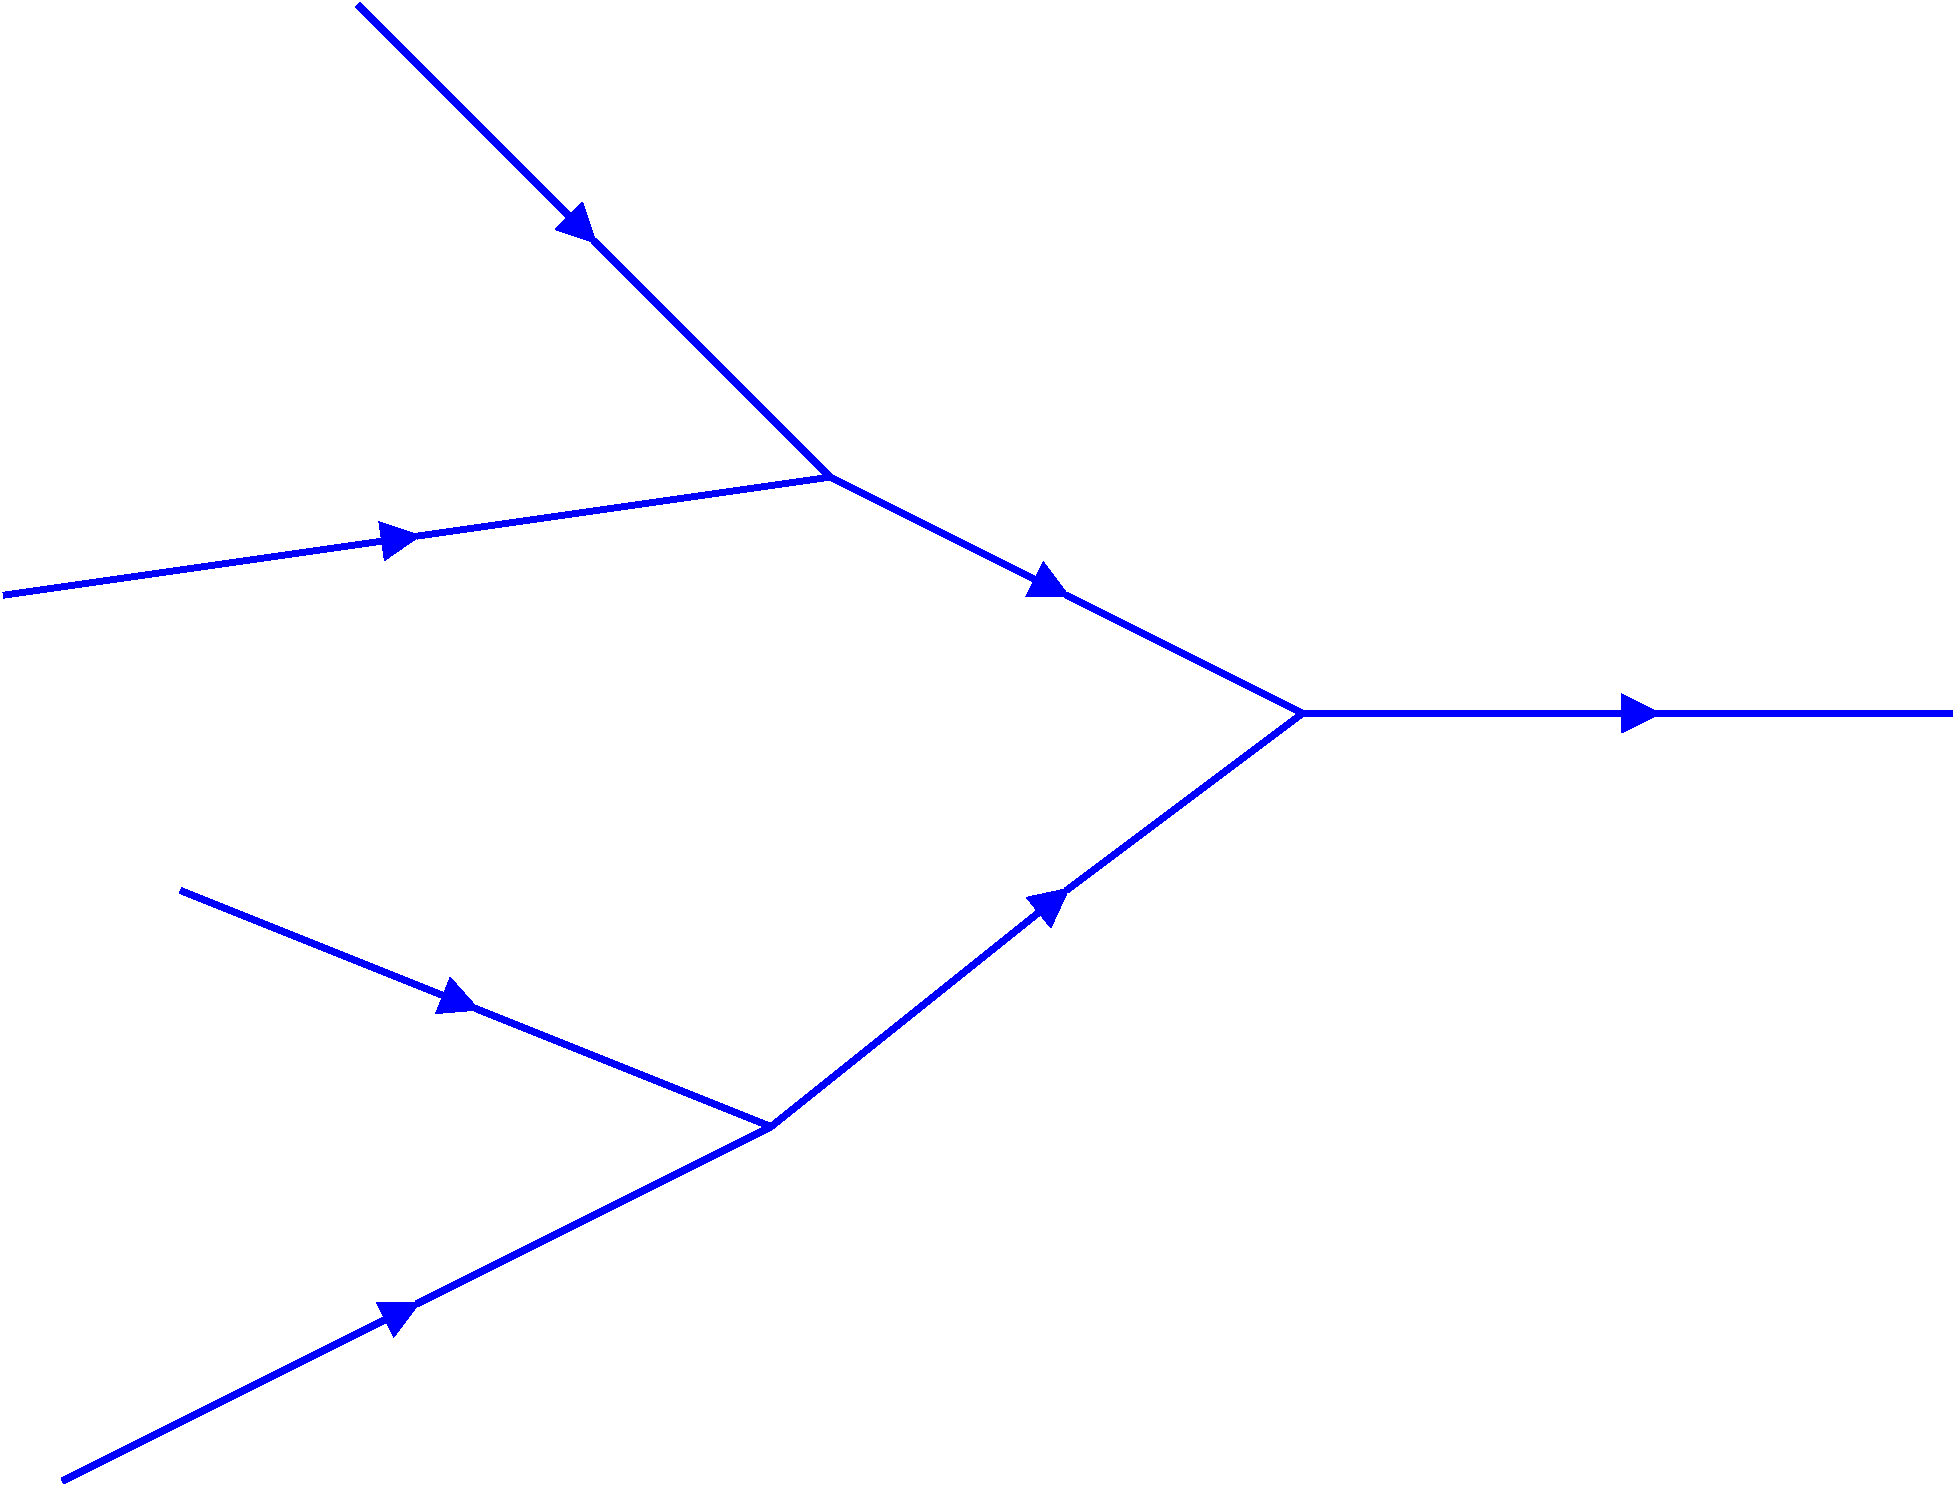
\includegraphics[width=0.6\columnwidth]{figures/stream_next_edge}
    \caption{Stream segmentation procedure network connectivity}
    \label{fig:stream_next_edge}
  \end{center}
\end{figure}

On the top of GRASS GIS provider a specialized GRASS {\em r.smoderp2d}
module has been designed. This tool allows a user running SMODERP2D
model computation directly from GRASS GIS working environment as
+demostrated in Figure~\ref{fig:r.smoderp2d}. The module can be easily
installed in GRASS GIS similarly to other extensions (so-called addons
modules) by {\em g.extension} command. By default, the {\em
  r.smoderp2d} module performs data preparation phase followed by
model computation steps. Data preparation only can be performed by
{\em -d} flag. In this case, the module creates a binary pickle file
which can be later used for a subsequent model computation. Note that
ArcGIS Toolbox also allows creating a pickle file for later
usage. Importantly, such pickle files are platform independent.

\begin{figure}[ht!]
  \begin{center}
    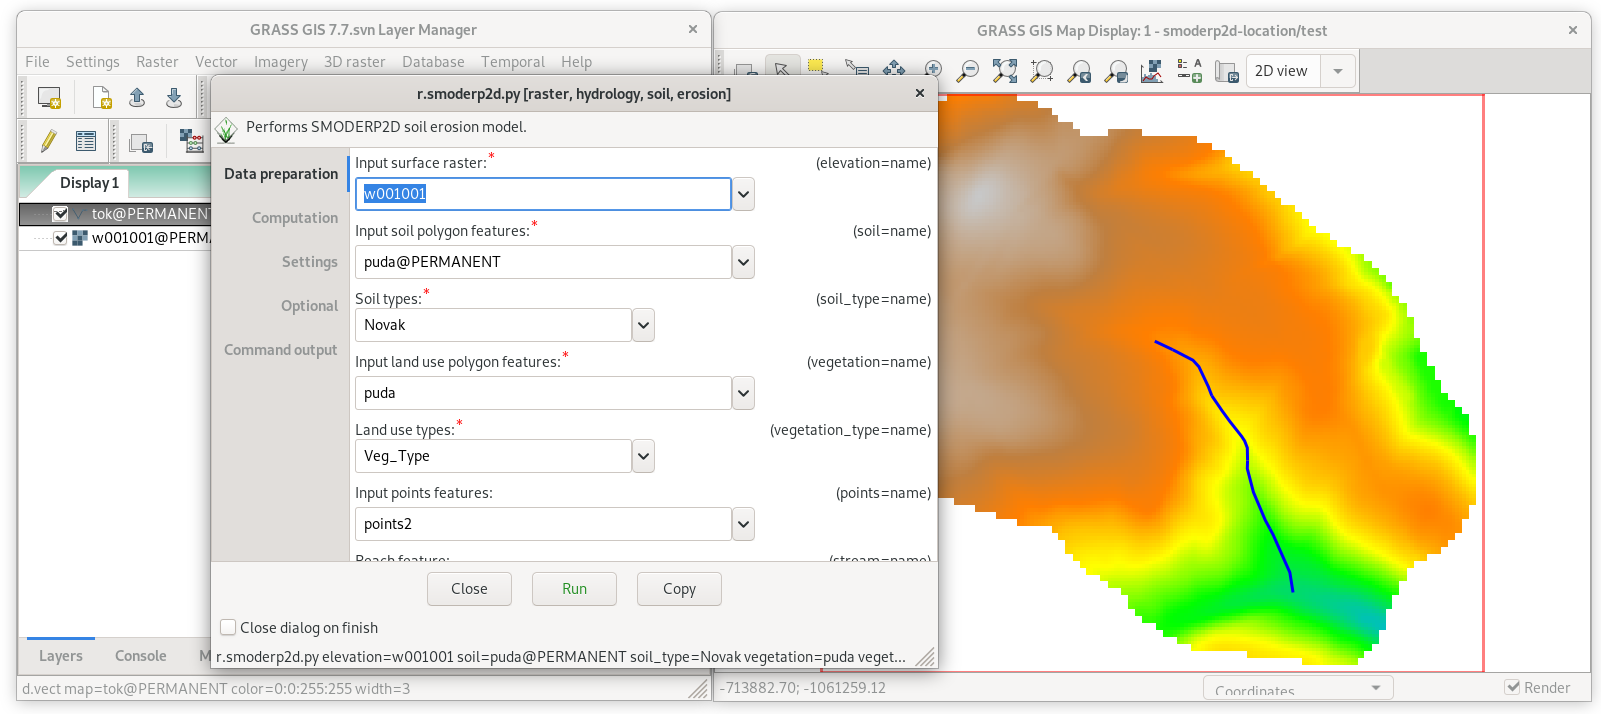
\includegraphics[width=1.0\columnwidth]{figures/smoderp2d_grass.png}
    \caption{Running r.smoderp2d module from GRASS GIS graphical user interface}
    \label{fig:r.smoderp2d}
  \end{center}
\end{figure}

{\em r.smoderp2d} command-line usage example:
\begin{verbatim}
r.smoderp2d elevation=w001001 soil=soil_map \
 soil_type=Novak vegetation=soil_map \
 vegetation_type=veg rainfall_file=rainfall.txt \
 points=points2 table_soil_vegetation=tab_sv \
 table_soil_vegetation_code=soilveg \
 table_stream_shape=tab_stream_shape \
 table_stream_shape_code=smoderp stream=stream 
\end{verbatim}

\subsubsection{QGIS plugin}
Recently the SMODERP2D model has been integrated also into QGIS
environment. QGIS\footnote{https://www.qgis.org} is a widely used open
source GIS platform which can be easily extended by user-defined
plugins. A SMODERP2D QGIS plugin allows performing both data
preparation and model computation phases in QGIS native environment,
see Figure~\ref{fig:smoderp2_qgis}. Data preprocessing is ensured by
GRASS GIS provider as described in \ref{sec:grass_provider}. Note that
QGIS installation normally comes with GRASS GIS included. It means
that GRASS dependency is solved by QGIS installation
itself. Experimental code of the plugin compatible with the current
long term release QGIS version 3.4 is available from the project GitHub
repository \cite{smoderp2d-github-2019}.

\begin{figure}[ht!]
  \begin{center}
    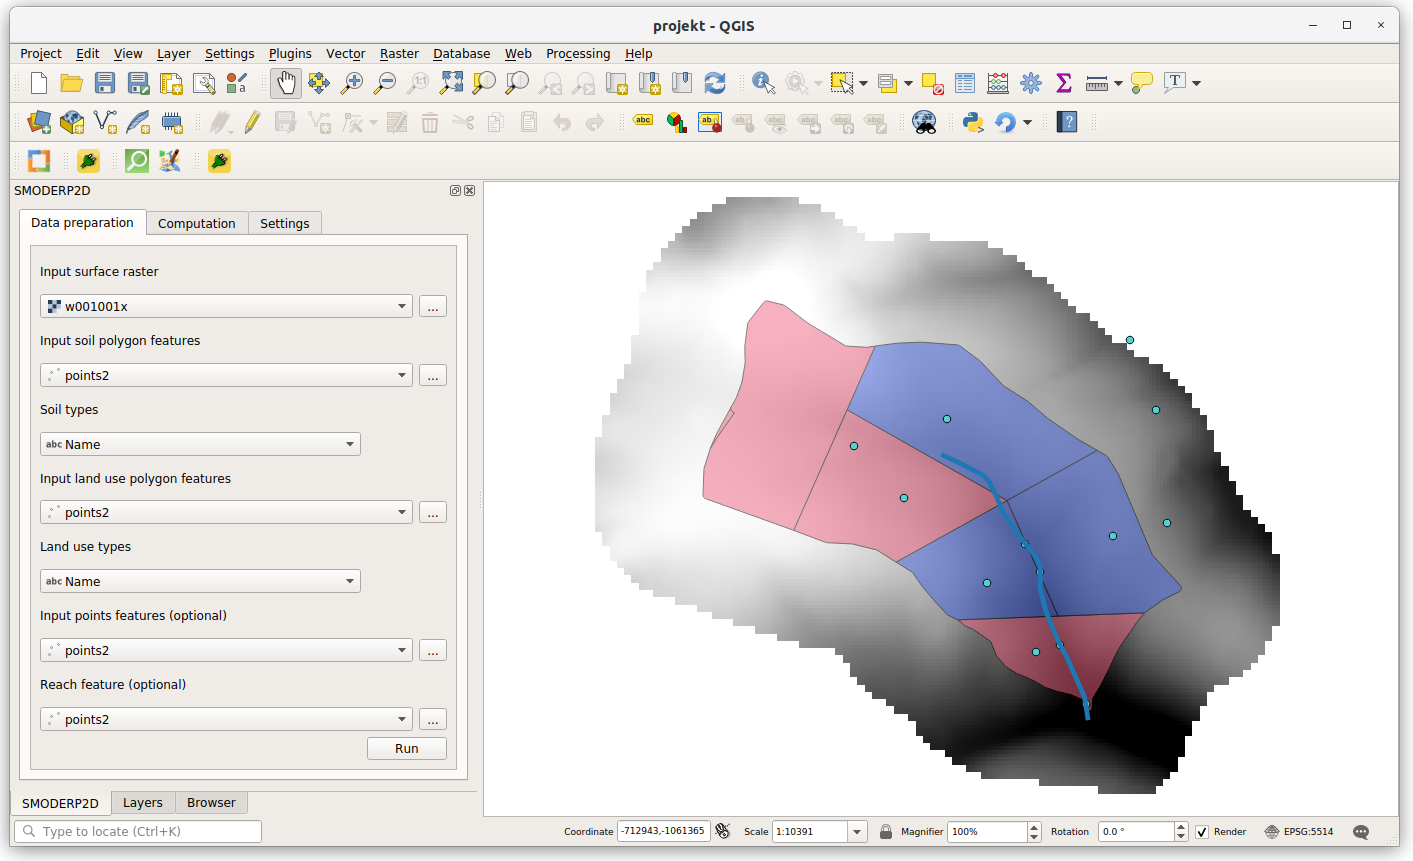
\includegraphics[width=1.0\columnwidth]{figures/smoderp2d_qgis.png}
    \caption{SMODERP2D model implemented as QGIS plugin}
    \label{fig:smoderp2_qgis}
  \end{center}
\end{figure}

\subsubsection{Python3 support}
SMODERP2D project also comes with Python 3 support, but still
supporting Python 2. Note that Python versions 2 and 3 are not
backwards compatible.  Python~3 support is important from various
perspectives. Python 2 is slowly reaching the end of
life\footnote{https://legacy.python.org/dev/peps/pep-0373/}, but is still used by many GIS platforms such as Esri ArcGIS 10.x. Newly supported
GIS platforms by the SMODERP2D project as Esri ArcGIS Pro, (upcoming)
GRASS GIS 7.8 and QGIS 3.x are Python 3 based. On the other hand it is
still meaningful to support both Python versions, Python 2 mainly
because of Esri ArcGIS 10.x platform.

\begin{figure}[ht!]
  \begin{center}
    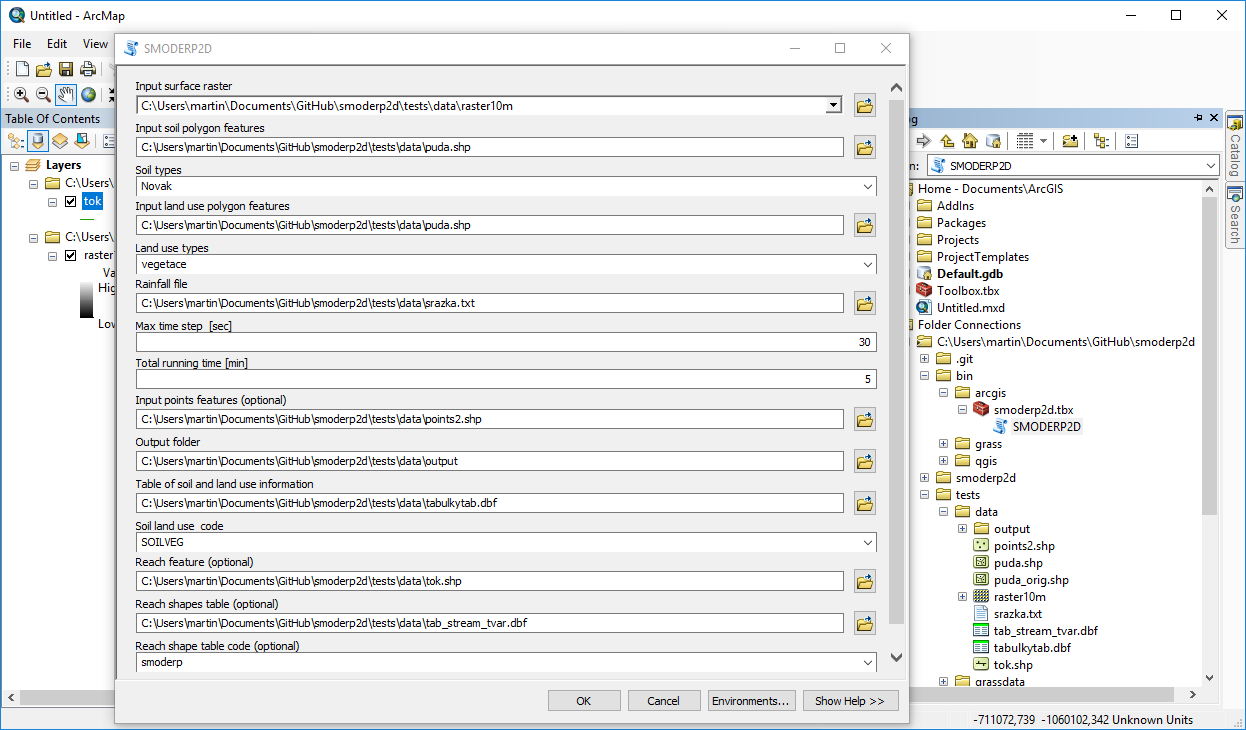
\includegraphics[width=1.0\columnwidth]{figures/smoderp2d_arcgis.png}
    \caption{SMODERP2D model available as ArcToolbox for Esri ArcGIS
      10.x and Pro platforms}
    \label{fig:smoderp2d_arcgis}
  \end{center}
\end{figure}


\subsection{Parallel computing experiments}

Because one of the most crucial points of SMODERP2D computations is
the speed, an experimental branch allowing (both CPU and GPU-based)
parallelised computations has been developed.

The main step was to rewrite all loop-based computations into
matrix-based mathematical operations. To keep matrices as so-called
tensors and to perform all the operations, an open source  TensorFlow Python
library \cite{tensorflow2015-whitepaper} developed by Google Brain
Team\footnote{https://ai.google/research/teams/brain/} was used. Even though
TensorFlow is most widely used for machine learning
and its performance on basic mathematical operations is not always better
than the one of NumPy (a quick comparison with NumPy and Numba can be
seen in \cite{tf-np}), it had been preferred for its easy switch
between CPU and GPU-based core (it depends only on the version of
TensorFlow the user has installed, no needs for changes in the code) and
therefore support also for users without an access to machines with
GPU. Another advantage of TensorFlow is its usage of so-called
graphs. A graph is a representation of all operations in
dataflow/workflow. Its individual operations are automatically sent
to multiple cores in a CPU or multiple threads in a GPU. These nodes
are run independently in parallel.

To support further development of TensorFlow and exploit its bleeding
edge functionalities, TensorFlow 2.0, which is published currently
just as an alpha version, was used in the SMODERP2D experimental
branch. Because TensorFlow 2.0 is still not suitable with all the
Python acrobatic tricks, NumPy was used for matrix operations in
places where TensorFlow could not (on places where loops were still
needed; looping through a NumPy array is incomparably faster than
through a~Tensor).

This experimental SMODERP2D branch is still under development;
however, the alpha-version is ready to be used. Table \ref{tab:GPU_results}
presents the results of different tests made on this version
(comparing parallelized GPU computation, parallelized CPU computation and a single CPU one).

\begin{table}[h]
  \centering
  \caption{Results of parallelization tests}
  \makegapedcells
  {\small
  \begin{tabular}{|l|p{2.2cm}|c|c|}\hline
    RAM & Processing unit & Data 62 KB & Data 197 MB\\
     & & [s] & [s]\\\hline
    \multirow{3}{*}{15 GB} & GPU1 & 4.0 & 7,560\\
    & CPU1 & 0.2 & 12,809\\
    & CPU2 & 2.1 & 7,249\\\hline
    \multirow{3}{*}{251 GB} & GPU2 & 2.5 & 6,611\\
    & CPU3 & 0.2 & 10,637\\
    & CPU4 & 1.5 & 8,631\\\hline
  \end{tabular}
  \vskip 2em
  \label{tab:GPU_results}
  \caption{Used processing units}
  \begin{tabular}{|l|p{2.5cm}|c|c|}\hline
    ID & Model & Clock speed & Memory\\\hline
    GPU1 & GeForce GTX 1060 3GB & 33 MHz & 3,016 MiB \\\hline
    GPU2 & $4\times$ GeForce GTX 1080 Ti & 33 MHz & 11,178 MiB \\\hline
    CPU1 & AMD Ryzen 7 1700 Eight Core Processor & 1.373 GHz & 512 KB \\\hline
    CPU2 & $16\times$ AMD Ryzen 7 1700 Eight Core Processor & 1.373 GHz & 512 KB \\\hline
    CPU3 & Intel Xeon CPU E5-2630 v4 & 2.4 GHz & 25,600 KB \\\hline
    CPU4 & $40\times$ Intel Xeon CPU E5-2630 v4 & 2.4 GHz & 25,600 KB \\\hline
  \end{tabular}
  }
\end{table}

As can be seen in the table, the usage of GPUs is not always
the~right way even when compared with CPUs, both single and parallelized ones.
The bottleneck of TensorFlow is its graph initialization; this step is very
time-consuming and therefore can last many times longer than the computation
itself for extremely small data. Another bottleneck is the memory shift between RAM and GPU virtual memory which concludes into slower processes for weaker GPUs (compared with parallelized computations being run on CPUs). Generally, for data of common size
was the process with parallelized computations faster (reaching around 60 per cent of the total
computation time on different architectures). Interesting moment is slower run of much stronger $CPU4$ when compared with weaker $CPU2$; this behaviour has to be examined deeper. 

\subsubsection{Further ideas for a sub-basins based parallel computing}
Besides the GPU-based parallelization (with TensorFlow \cite{tensorflow2015-whitepaper} or
NVIDIA Cuda technology~\cite{Kalyanapu2011,Le2015}) the
pure CPU parallelization may also bring a good improvement in the computation
time reduction. The computation domain is separated into sub-domains
based on a certain algorithm where each sub-domain computation is loaded to a single
CPU core.  It is beneficial to incorporate the
hydrological behaviour in the parallelization
strategy if the domain is a hydrological basin. 
In~\cite{Vivoni2011} the basin was separated in sub-basins
based on stream network. The sub-basins communicated with each other through so-called
ghost cell. The strategy aimed to generate as few ghost cells as
possible; to reduce the communication between the CPU cores. 

The parallelization strategy outlined in the manuscript is based on
the hydrological reality and it is shown in a simplified setup in Figure~\ref{fig:cpu-parallel}. In this example, the Nu\v{c}ice experimental catchment
was chosen to present the parallelization strategy. At this 0.5 km$^2$ large 
basin a long-term monitoring of erosion and runoff processes is being conducted 
by the Dept.\ of Landscape Water Conservation. 

\begin{figure}[ht!]
  \begin{center}
    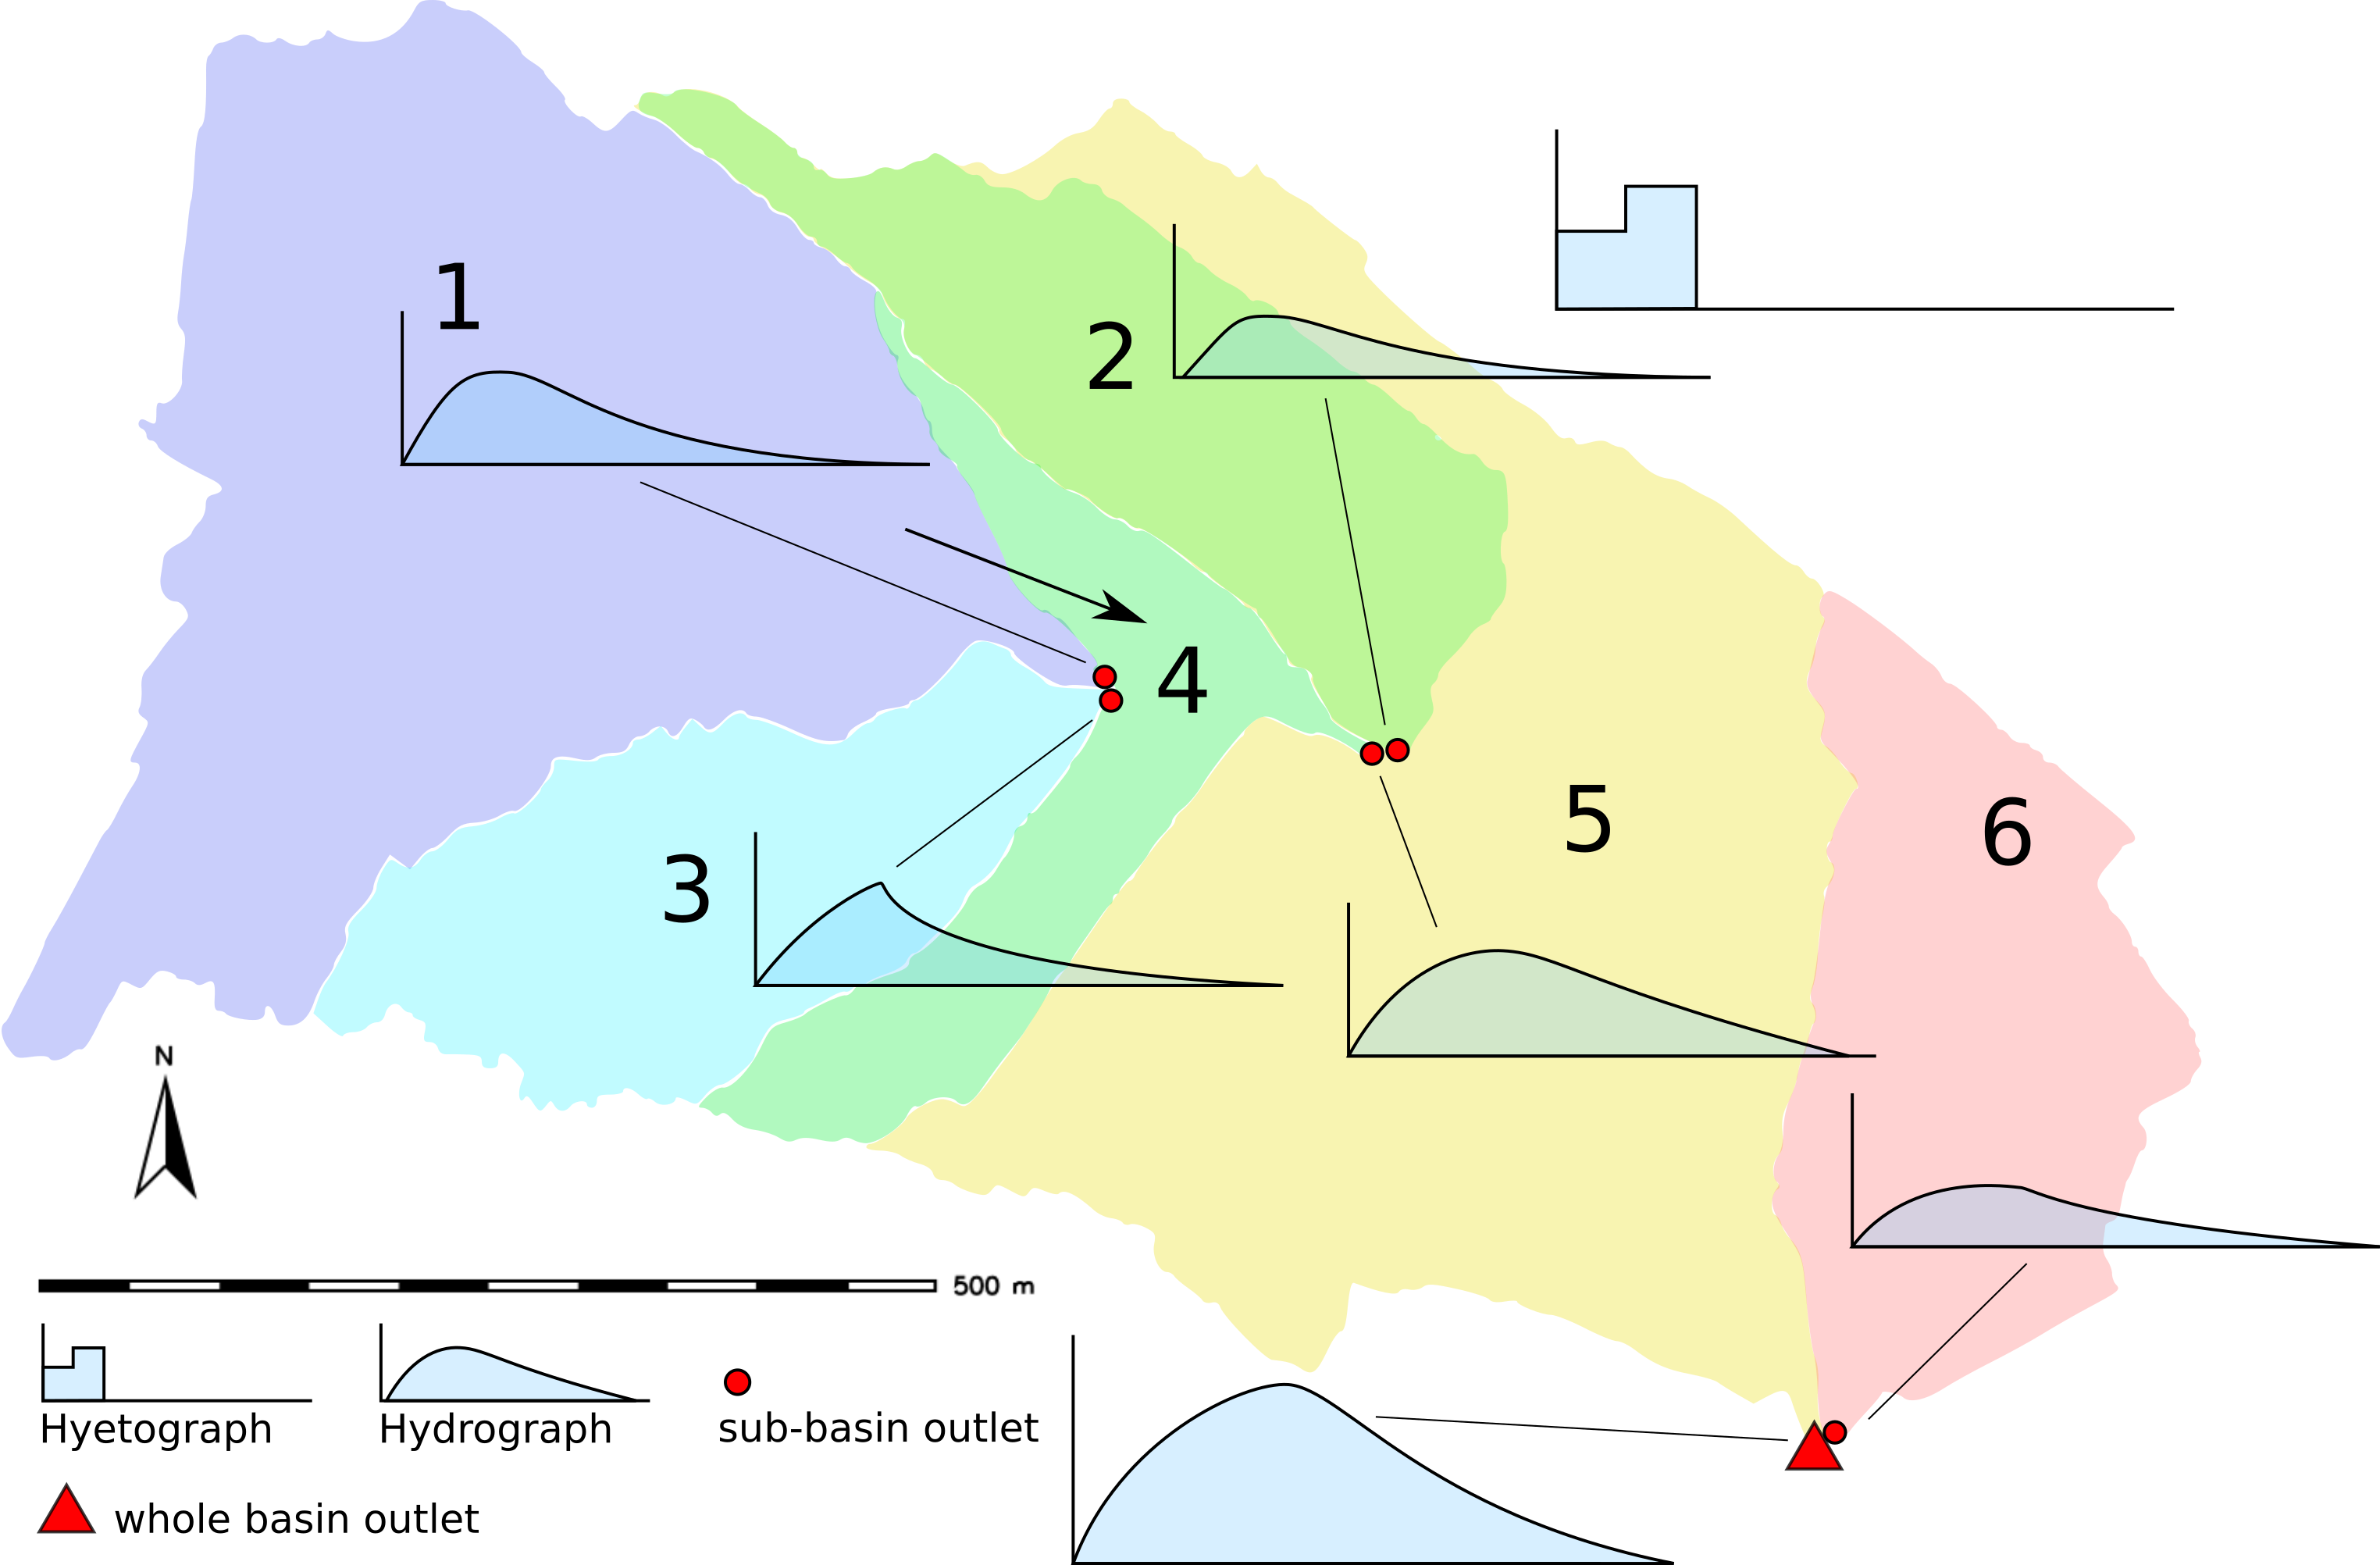
\includegraphics[width=0.9\columnwidth]{figures/smoderp-cpu-parallel.png}
    \caption{Simple example of possible CPU-based parallelization strategy for the experimental catchment Nu\v{c}ice}
    \label{fig:cpu-parallel}
  \end{center}
\end{figure}

The strategy main goal is the reduction of
the communication between CPU-cores during the computation as much as
possible. The whole basin is divided into several sub-basins based on
the digital elevation model and user-defined sub-basin size. 
Outlet\footnote{The location in the basin where all water from the basin flows} 
of each sub-basin is depicted with
red dots in Figure~\ref{fig:cpu-parallel}. After the sub-basins
are defined, an order in which each sub-basin will be computed is defined as
follows. Sub-basins which are hydrologically the farthest from the
basin outlet (depicted by the triangle in Figure~\ref{fig:cpu-parallel}) 
and therefore have no inflow flow upslope area are
calculated at first. Those sub-basins have the rainfall stored in
hyetographs as the only input. In the simplified setup shown in
Figure~\ref{fig:cpu-parallel}, the sub-basins 1, 2, 3, and 6 are
calculated at first in parallel. The calculated hydrographs of the
sub-basins 1, 2, 3, and 6 are stored in the memory for the later use. 
Sub-basins which have sub-basins 1, 2, 3, and 6 in its upslope area 
are calculated next. 
It this case it is the only the sub-basin 4. The water inputs in
the sub-basin 4 are now hyetograph and also hydrographs of
upslope sub-basins 1 and 3. 
Next sub-basin to be calculated is the final sub-basin 5. 
In this sub-basin is the outlet of the whole area.
The water input in the final sub-basin 5 are hyetograph and hydrographs 
of sub-basins 2, 4 and 6. Once the main outlet hydrograph is obtained 
the calculation stores the results and stops. 

This approach may encounter several limitations. The main one
originates from the basin geometry. In the case of a narrow basin
situation (each sub-basin has a single upslope and downslope
sub-basin), the sub-basins will be computed in a sequence, which loses
the advantage of multi-core working station. If this situation happens
the user will be forced to create very small sub-basins in order to be
able to perform the outlined CPU parallelization. The possibilities of
CPU parallelization described in this section will be the subject of
further research.


\section{CONCLUSION}

This manuscript presents SMODERP2D project and recently triggered 
development. Complete SMODERP2D source code is available on GitHub 
\cite{xxx} under GNU GPL licence. SMODERP2D computational tools have 
been successfully integrated into Esri ArcGIS, GRASS GIS and QGIS desktop GIS platforms. On top of that, the concept of so-called GIS providers allows publishing the SMODERP2D model as web processing service. Establishing experimental SMODERP2D 
OGC Web Processing Service is planned for 2019. Ongoing development 
is mainly focused on computational routines and parallel computations experiments. All the tools are currently distributed as experimental and are available for testing and user feedback.
The~official stable release of SMODERP2D model is planned in 2020. This 
includes also user documentation which is currently under development. 
In the 
case of SMODERP2D model, the run-time is an issue, especially 
if multiple mid-scale hydrological basins in fine spatial 
resolution grid computation needs to be undertaken. The code parallelization
is a common practice in cases where 
the reduction of run-time is convenient or even necessary, therefore
the existence of the TensorFlow-based branch; and although this branch is still
under development, the reduction of the computation costs is already reaching up to 40 per
cent depending on the data and architecture. This experiment also shows that the parallelized branch should not be used as the default one, but an ad hoc solution should be chosen depending on the data and available computing power. Even 
though the SMODERP2D model does not belong in the family of forecasting 
models (where the short run-time is necessary)  the run-time speed 
up will increase the usability of the model in practice and research applications. 


\section*{ACKNOWLEDGEMENTS}\label{ACKNOWLEDGEMENTS}
The research has been supported by the research grants TJ01000270,
QK1910029, and internal CTU grant SGS17/173/OHK1/T3/11.

{
  \begin{spacing}{1.17}
    \normalsize
    \bibliography{smoderp2d_foss4g_2019} % Include your own bibliography (*.bib), style is given in isprs.cls
  \end{spacing}
}

\vspace{1cm}
\textit{Revised April 2019}

\end{document}
